\documentclass{article}
\usepackage{xfrac,amsmath,amsthm,amssymb,parskip,enumitem,url}
\usepackage[numbers,sort&compress]{natbib}

\newtheorem{definition}{Definition}
\newtheorem{construction}{Construction}
\newtheorem{theorem}{Theorem}

\newcommand{\oprf}[0]{\mathsf{OPRF}}
\newcommand{\getr}[0]{\stackrel{\$}{\leftarrow}}
\newcommand{\enc}[0]{{\mathsf{Enc}}}
\newcommand{\dec}[0]{{\mathsf{Dec}}}
\newcommand{\fixme}[1]{{\bf{}\ [FIXME:} {\emph{#1}} {\bf{}]}}
\newcommand{\todo}[1]{{\bf ToDo:} {{\bf #1}}}
\newcommand{\dash}[0]{{\text -}}
\newcommand{\A}[0]{{\mathcal{A}}}


\newcommand{\myO}[0]{\mathcal{O}}
\newcommand{\ioprf}[0]{\mathsf{i}\mathsf{OPRF}}
\newcommand{\iprf}[0]{\mathsf{i}\mathsf{PRF}}
\newcommand{\ot}[0]{\mathsf{OT}}
\newcommand{\proto}[0]{{\pi_{\ioprf}}}
\newcommand{\myS}[0]{{\mathcal{S}}}
\newcommand{\myF}[0]{{\mathcal{F}}}
\newcommand{\Z}[0]{\mathbb{Z}}
\newcommand{\G}[0]{\mathbb{G}}
\newcommand{\Hide}[1]{}

\newcommand{\prg}[0]{\mathsf{PRG}}
\newcommand{\seed}[0]{\mathsf{seed}}
\newcommand{\myroot}[0]{\mathsf{ROOT}}

\newcommand{\trace}[0]{\mathsf{Trace}}
\newcommand{\crs}[0]{\mathsf{CRS}}
\newcommand{\com}[0]{\mathsf{com}}
\newcommand{\sr}[0]{{\stackrel{?}{=}}}

\let\ignore\Hide

\newcommand{\N}[0]{{\mathbb{N}}}

\makeatletter
\def\old@comma{,}
\catcode`\,=13
\def,{%
  \ifmmode%
    \old@comma\discretionary{}{}{}%
  \else%
    \old@comma%
  \fi%
}
\makeatother



\begin{document}
\title{Iterative Oblivious Pseudo-Random Functions and Applications}
\author{}\date{}
\maketitle

\section{ToDo}
\begin{itemize}
\item Tightness in the PRF proof
\item \emph{Iterative} PRF or \emph{Iterated} PRF?
\item Proof of security for $\proto$. And: delegation. And: proof of one-sided security, and: verifiability.
\item Implementation
\item Decision tree application?  
\end{itemize}

Advantages: fully malicious security (not HVZK!) and verifiability,
delegation

\begin{abstract}
x
\end{abstract}
\section{Introduction}
Structured encryption allows a data owner to encrypt structured data,
and outsource it to an untrusted server.  They crucial property of
structured encryption is that the data owner can later compute a
special decryption key for the server which permits the server to
decrypt and parse a well defined component of the data structure.  A
typical example for structured data is data arranged in a graph, and
the owner computes keys for decryption of sub-graphs.  Computation of
decryption keys is possible despite the owner retaining only a
constant-sized master key.

In this paper, we introduce a twist to the standard setting of
structured encryption. Another party, the client, can ask the data
owner to compute a key to decrypt a specific component of the owner's
data structure. Yet, data owner and client are mutually
untrusted. That is, the client does not want to reveal to the
(potentially) fully-malicious owner which component of the data
structure the client is interested in. The owner wants to prepare a
decryption key which confines the (potentially) fully-malicious client
to decrypting only data from one component of the data
structure. Using the decryption key, the client then fetches the
component of the data structure they are interested in from the server
and decrypts it. In case the client does not trust the server, the
client reverts to standard techniques such as PIR to fetch data from
the server.

We focus only on directed acyclic graph data structures, i.e., trees,
but in return offer more powerful confinement control than structured
encryption for the data owner.  In addition to decryption keys
enabling decryption of a sub-tree for the client, the data owner can
also compute keys which enable the client to access only one path,
from the root of the tree to a leaf.  Moreover, the client can ask to
decrypt a path in an iterative, adaptive fashion instead of querying
the owner at once.  That is, the client will parse the tree node by
node, obliviously asking the owner to decrypt the next node in the
tree only after fetching and decrypting the previous node.  For
example, after decrypting one node of a binary tree, the client can
obliviously query the owner for the decryption key of either the left
or right child, depending on the current node's data content.  At the
same time, the data owner wants to ensure that the client can only ask
to decrypt a node which is a child of the current node, such that the
client is confined to decrypting exactly one path and cannot
arbitrarily ``jump around'' in the data structure.  We will see later
that our new setting of structured encryption for trees with an
untrusted client has several interesting real-world applications.

Yet, enabling this new scenario turns out to be technically
challenging.  A straightforward, intuitive approach might be for the
owner to apply an Oblivious Pseudo-Random Function (OPRF) as the PRF
to encrypt nodes. For a tree of height $\ell$, owner and client then
run $\ell$ instances of the OPRF such that the client always learns
the key for the next node on the path they are interested in, and the
owner learns nothing. However, this approach is only secure against
semi-honest clients which stick to the rule of asking for the
decryption key of one child node of the current node. The difficulty
lies in making parsing the tree structure secure against a
fully-malicious client without reverting to general, yet expensive
techniques such as maliciously secure two-party computation and
expensive general Zero-Knowledge Proofs.

Consequently, we introduce the notion of iterated Oblivious
Pseudo-Random Functions ($\ioprf$s) and introduce candidate
constructions. An $\ioprf$ is an $\ell$ round two party protocol
between a sender and a receiver. Its definition captures the intuition
that the receiver can adaptively query $\ell$ input bits $x_i$ in
$\ell$ rounds such that in the end they learn outputs
$\text{PRF}_K(x_1),\ldots,\text{PRF}_K(x_1\ldots{}x_\ell)$ for key $K$
chosen by the sender, and the sender learns nothing.

Our $\ioprf$ construction is based on a careful adoption of the PRF by
\citet{prf}. We first augment the \citeauthor{prf} PRF to become an
iterated Pseudo-Random Function ($\iprf$) which has the property that,
for input strings with the same prefix, its generated output also
shares the same prefix. We then use the same trick as \citet{oprf} to
convert the $\iprf$ to an $\ioprf$. This first $\ioprf$ is OT-based
and thus very efficient, yet it only offers one-sided security with a
malicious receiver and semi-honest sender. We then present our main
construction, an $\ioprf$ which is secure against malicious sender and
malicious receiver. We achieve malicious security by designing
efficient zero-knowledge proofs for DH-based statements over elliptic
curves.

\todo{continue, main contributions, implementation}

\section{$\ioprf$ Background}
NOTE: for one-sided security, we use the OT-based solution.

\todo{Add description that PRF outputs must be hashed to become real
  output of the PRF. This is necessary for the leftover hash lemma.}


\begin{definition}[$\iprf$]\label{defiprf}
  For keys $K=(K_1,\ldots,K_\ell)\in\{0,1\}^{\ell\cdot\lambda}$ and
  inputs $x=(x_1\ldots{}x_\ell)\in\{0,1\}^\ell$, an iterated
  pseudo-random function family $\iprf_{K}(x)$ is a sequence of
  function families
  $(f^1_{K_1}(x_{1}),\ldots,f^\ell_{K_1,\ldots,K_\ell}(x_{1}\ldots{}x_{\ell}))$,
  where each
  $f^i_{K_1,\ldots,K_i}(x_{1}\ldots{}x_{i}):\{0,1\}^{i\cdot\lambda}\times\{0,1\}^{i}\rightarrow{}v_i\in\{0,1\}^\lambda$
  is a pseudo-random function family with keys $(K_1,\ldots,K_i)$ from $K$ and
  inputs $(x_1\ldots{}x_i)$ from $x$.
\end{definition}

\paragraph{Remarks}
An implication of Definition~\ref{defiprf} is that probability
ensemble (family of random variables)
$V_\lambda=(v_1,\ldots,v_\ell)=\iprf_K(x)\in\{0,1\}^{\ell\cdot\lambda}$
is computationally indistinguishable from the probability ensemble
$U_\lambda$ describing uniformly random bit strings of length
$\lambda$.

A simple real-world construction for an $\iprf$ is based on variable
length PRFs, such as HMAC, and a collision resistant hash function
$H$. For example, consider
$\iprf_K(x)=(\hmac_{H(K_1)}(x_1),\ldots,\hmac_{H(K_1||\ldots||K_\ell)}(x_1\ldots{}x_\ell))$.


\begin{figure}[tb]
\RestyleAlgo{boxed}
\LinesNumbered
\begin{functionality}[H]
$S\rightarrow{}\fioprf$: $K$\;
\For{$i=1$ {\bf to} {$\ell$} }{
  $R\rightarrow{}\fioprf:x_i$\;
  $\fioprf\rightarrow{}R: v_i$ such that $(v_1,\ldots,v_\ell)=\iprf_K(x_1\ldots{}x_\ell)$\;
}
\end{functionality}
\caption{Functionality $\fioprf$\label{idealioprf}}
\end{figure}

\begin{definition}[$\proto$]
  An iterated \emph{oblivious} pseudo-random function is an
  $\ell$-round probabilistic protocol $\proto$ between a sender $S$
  with input key $K\in\{0,1\}^{\lambda\cdot\ell}$ and receiver $R$
  with input bit string $x=(x_1\ldots{}x_\ell)\in\{0,1\}^{\ell}$ with
  the following properties.

  \begin{itemize}
   
  \item Protocol $\proto$ realizes the ideal functionality $\fioprf$
    shown in Figure~\ref{idealioprf}. After $\ell$ rounds, $R$ has
    received $(v_1,\ldots,v_\ell)=\iprf_K(x),|v_i|=\lambda$ from
    $\fioprf$, where $\iprf_K$ is an iterated pseudo-random function
    family. Sender $S$ receives nothing from $\fioprf$.
  
  \item For all adversaries $\A$ in the real world, there exists a
    simulator $\myS_R$ in the ideal world such that $R$'s view
    $\mathsf{REAL}_{\proto,\A,R}(x,K)$ in the real world is
    computationally indistinguishable from $R$'s view
    $\mathsf{IDEAL}_{\fioprf,\myS_R(x)}(x,K)$ in the ideal world.

  \item For all adversaries $\A$ in the real world, there exists a
    simulator $\myS_S$ in the ideal world such that $S$'s view
    $\mathsf{REAL}_{\proto,\A,S}(K)$ in the real world is
    computationally indistinguishable from $S$'s view
    $\mathsf{IDEAL}_{\fioprf,\myS_S}(K)$ in the ideal world.
\end{itemize}
\end{definition}

The crucial property of $\fioprf$ in contrast to standard $\oprf$s is
that $R$ can oblivious evaluate a PRF a total of $\ell$ times, but not
on arbitrary inputs. In each round $i$, $R$ submits input $x_i$, but
the PRF will be evaluated using $R$'s previous input
$x_1\ldots{}x_{i-1}$ as a prefix.

\todo{Introduce delegatable PRFs}

\section{Constructions}
We present new constructions for both $\iprf$ and $\ioprf$.  To ease
readability, we omit an important technicality in the description and
proofs: our $\iprf$ and $\ioprf$ construction do not output
pseudo-random bit strings of length $\lambda$, but pseudo-random
elements of DDH group $\G$. Yet, converting elements to bit strings
follows from a standard application of the leftover hash
lemma~\cite{leftover}. So in the following, assume that
$|\G|\ge{}2^\lambda$, and each party implicitly hashes the output of
$\iprf$ and $\ioprf$ using any pairwise independent family of hash
functions.




\subsection{$\iprf$ Construction}
Let $\G$ be a group of prime order $p$ where the DDH assumption holds,
and $g$ is a random generator of $\G$.

Initialization: choose a key $K=(\vec{{\alpha}},\vec{\beta})$ by sampling
$\ell$ pairs of random scalars
${\alpha_{i}},{\beta_{i}}\getr\Z_p.$

$\iprf(x_1,\ldots,x_\ell)$: output a vector $\vec{v}$ of length $\ell$ where $v_i = g^{\prod_{j=1}^{i} (\alpha_jx_j+\beta_j(1-x_j))}.$

\todo{Show that this is a delegatable PRF.}


\subsubsection{Dual-PRF is still a PRF}

\begin{construction} 
Define the function ensemble $F = \{F_n\}_{n\in N}$.  For every $n$, a key of a function $F_n$ is a tuple, $\langle P,Q,g,\vec{\alpha}\rangle$, 
where $P$ is an $n$-bit prime, $Q$ a prime divisor of $P-1$, $g$ an element of order $Q$ in $\mathbb{Z}_{p}^*$ and $\vec{\alpha}=\langle 
\alpha_0,\alpha_1, \ldots , \alpha_n \rangle$ a uniformly random sequence of $n+1$ elements of $\mathbb{Z}_Q$.  For any $n$-bit input, $x=x_1 x_2 \ldots x_n$, the 
function $f_{P,Q,g,\vec{\alpha}}$ is defined by:
 $$f_{P,Q,g,\vec{\alpha}}(x) = (g^{\alpha_0})^{\prod_{x_i=1}\alpha_i}$$
\end{construction}

\begin{theorem}
\label{theorem:naor}
If the DDH-Assumption holds, then for every probabilistic polynomial-time oracle machine $\mathcal{M}$, every constant $\gamma > 0$, and for all but a finite number of $n$'s
$$| Pr[\mathcal{M}^{f_{P,Q,g,\vec{\alpha}}}(P,Q,g)=1] - Pr[\mathcal{M}^{R_{P,Q,g}}(P,Q,g) = 1]| < \frac{1}{n^\gamma} $$
where in the first probability, $f_{P,Q,g,\vec{\alpha}}$ is distributed according to $F_n$, and in the second probability the distribution of $R_{P,Q,g}$ is uniformly chosen in the set of functions with the domain $\{0,1\}^n$ and range $\langle g\rangle$.
\end{theorem}

\begin{construction}
\label{const:newprf}
Define the function ensemble $F' = \{F'_n\}_{n\in N}$.  For every $n$, a key of a function $F'_n$ is a tuple, $\langle P,Q,g,\vec{\alpha},\vec{\beta}\rangle$, 
where $P$ is an $n$-bit prime, $Q$ a prime divisor of $P-1$, $g$ an element of order $Q$ in $\mathbb{Z}_{p}^*$ and $\vec{\alpha}=\langle 
\alpha_0,\alpha_1, \ldots , \alpha_n \rangle$ and $\vec{\beta}=\langle 
\beta_0,\beta_1, \ldots ,\beta_n \rangle$, uniformly random sequences of $n+1$ elements of $\mathbb{Z}_Q$.  For any $n$-bit input, $x=x_1 x_2 \ldots x_n$, the 
function $f'_{P,Q,g,\vec{a},\vec{b}}$ is defined by:
 $$f'_{P,Q,g,\vec{\alpha},\vec{\beta}}(x) = (g^{\alpha_0})^{\prod_{x_i=1}\alpha_i \prod_{x_i=0}\beta_i}$$
 \end{construction}
 
\begin{theorem}
\label{theorem:newprf}

If the DDH-Assumption holds, then for every probabilistic polynomial-time oracle machine $\mathcal{M}$, every constant $\gamma > 0$, and for all byt a finite number of $n$'s

$$| Pr[\mathcal{M}^{f'_{P,Q,g,\vec{\alpha},\vec{\beta}}}(P,Q,g)=1] - Pr[\mathcal{M}^{R_{P,Q,g}}(P,Q,g) = 1]| < \frac{1}{n^\gamma} $$

where in the first probability, $f'_{P,Q,g,\vec{a},\vec{\beta}}$ is distributed according to $F'_n$, and in the second probability the distribution of $R_{P,Q,g}$ is uniformly chosen in the set of functions with the domain $\{0,1\}^n$ and range $\langle g\rangle$.
\end{theorem}

\begin{proof}
We prove this by reduction, showing that if $\mathcal{M}$ exists that can distinguish between $f'$ and a random function, then we can build $\mathcal{M}'$ that can distinguish between $f$ and a random function.

First, assume that $\mathcal{M}$ exists that can violate the inequality from Theorem \ref{theorem:newprf}.  We create $\mathcal{M'}$ as follows.  First, $\mathcal{M}'$ creates and stores a uniformly random vector $\vec{\beta}$ as in Construction~\ref{const:newprf}.  $\mathcal{M}'$ then runs $\mathcal{M}$ as a subroutine.  Each time $\mathcal{M}$ queries the oracle for an evaluation on input $y$, $\mathcal{M}'$ does the following:

\begin{enumerate}
\item Query his own oracle for $z = f(y)$
\item Calculate $z' = z^{\prod_{y_i = 0} \beta_i}$
\item Returns $z'$ to $\mathcal{M}$
\end{enumerate}

$\mathcal{M}'$ outputs the same as $\mathcal{M}$.  If  $\mathcal{M}'$ is interacting with the function $f$, then the responses he gives to $\mathcal{M}$ will be identical to the real function $f'$, due to him being able to add in the extra $b$ components to the result.  If $\mathcal{M}'$ is interacting with a random function, then the responses he gives will be distributed identically to a random function.  Therefore, if $\mathcal{M}$ has a distinguishing advantage, so will $\mathcal{M}'$.
\end{proof}



\subsection{DH-based $\proto$ Construction}
NOTE: for one-sided security, we use the OT-based solution.
\fixme{Switch to additive notation}


\subsubsection{Preliminaries}
Let there be two generators $g_1,g_2$ of prime order $p$ DDH group
$\G$. Nobody knows the discrete log of one generator $g_i$ to the
basis of the other generator $g_{j\neq{}i}$.

\paragraph{Elgamal Encryption}
We will use additive Elgamal encryption with private keys $sk\in\Z_p$
and public keys $pk=g_1^{sk}$. Ciphertext $c$ to encrypt $m\in\Z_p$ is
$c=(c[0],c[1])=(g_1^r,pk^r\cdot{}g_2^m)\leftarrow\enc_{pk}(m)$, where
$r\getr\Z_p$.

\paragraph{Pedersen Commitments}
A Pedersen commitment $\com_{g}(m)\in\G$ to message $m\in\Z_p$ is defined as
$\com_{g}(m)=g_1^r\cdot{}g^m$, where $r\getr\Z_p$, and $g\neq{}g_1$ is
a generator of $\G$.  To open $\com_{g}(m)$, reveal $(m,r)$.


\subsubsection{$\proto$ Initialization}
The sender in $\proto$ knows the $\iprf$'s secret key
$K=(\alpha_1,\ldots,\alpha_\ell,\beta_1,\ldots,\beta_\ell)$ as before. For some input
string $x=(x_1\ldots{}x_\ell)$, we define the output of $\proto$ for
the receiver as
$\iprf_K(x)=g_2^{\prod_{i=1}^{\ell}(\alpha_i{}x_i+\beta_i(1-x_i))}$.

The receiver computes $V_0 \leftarrow\enc_{pk}(1)$ and
$D_0\leftarrow\enc_{pk}(0)$, sends them to the sender and proves that
these are encryptions of $1$ and $0$ (see \S\ref{poe} below). The
sender computes Pedersen commitments
$(\com_{g_2}(\alpha_1),\ldots,\com_{g_2}(\alpha_\ell),\com_{g_2}(\beta_1),\ldots,\com_{g_2}(\beta_\ell))$,
sends them to the receiver, and proves knowledge of plaintexts in ZK
(see \S\ref{pokop}).

\subsubsection{$\proto$ Iterative Processing in $\ell$ Rounds}
In round $i\in\{1,\ldots,\ell\}$, for sender's input bit $x_i$:
\begin{enumerate}
\item {\bf Shuffling:}
\begin{enumerate}
\item For input bit $x_i$, the receiver computes Pedersen commitment
  $\com_{g_2}(x_i)$ and proves that $x_i\in\{0,1\}$ (see
  \S\ref{pobit}). Similarly, the receiver computes $\com_{g_2}(1-x_i)$
  and proves that $(1-x_i)\in\{0,1\}$ (see \S\ref{pobit}). Finally,
  the receiver proves that the sum of plaintexts behind
  $\com_{g_2}(x_i)$ and $\com_{g_2}(1-x_i)$ equals $1$ (see
  \S\ref{pkseo}).


\item  The receiver chooses $r,r',r'',r'''\getr\Z_p$ and computes Elgamal ciphertexts
  \begin{align*}
    &c_i=(g_1^r\cdot{}V_{i-1}[0]^{x_i},pk^{r}\cdot{}V_{i-1}[1]^{x_i})
    \\&c'_i=(g_1^{r'}\cdot{}V_{i-1}[0]^{1-x_i},pk^{r'}\cdot{}V_{i-1}[1]^{1-x_i})
    \\&d_i=(g_1^{r''}\cdot{}D_{i-1}[0]^{x_i},pk^{r''}\cdot{}D_{i-1}[1]^{x_i})
    \\&d'_i=(g_1^{r'''}\cdot{}D_{i-1}[0]^{1-x_i},pk^{r'''}\cdot{}D_{i-1}[1]^{1-x_i})%\text{ and}
  \end{align*}
  and sends $(c_i,c'_i,d_i,d'_i)$ to the sender.

\item The receiver proves correctness of the above computations in
  ZK. Specifically, $(c_i,c'_i,d_i,d'_i)$ result from correct
  exponentiation with $x_i$ (or $1-x_i$) from $\com_{g_2}(x_i)$ (or
  $\com_{g_2}(1-x_i)$), and multiplication with a random power of
  $g_1$ and $pk$, i.e., re-randomization (homomorphic addition of
  encryption of $0$).  See \S\ref{pshuffle} below for details.

   Both parties can now compute
    \begin{align*}&T_i=(c_i[0]\cdot{}d'_i[0],c_i[1]\cdot{}d'_i[1])
    \\&U_i=(c'_i[0]\cdot{}d_i[0],c'_i[1]\cdot{}d_i[1]).
    \end{align*}
   
  \end{enumerate}

\item {\bf PRF:} The sender computes Elgamal ciphertexts
  \begin{align*}
&X_i=(T_i[0]^{\alpha_i},T_i[1]^{\alpha_i})
\\&Y_i=(U_i[0]^{\beta_i},U_i[1]^{\beta_i}),
  \end{align*}
sends $(X_i,Y_i)$ to the receiver and proves correct exponentiation
(multiplication of plaintexts) in ZK (see \S\ref{pomult}).

\item {\bf Shuffling back:}
  For $r,r',r'',r'''\getr\Z_p$, the receiver computes
  \begin{align*}
    P_i&=(g_1^r\cdot{}X_i[0]^{x_i},pk^r\cdot{}X_i[1]^{x_i})
    \\P'_i&=(g_1^{r'}\cdot{}X_i[0]^{1-x_i},pk^{r'}\cdot{}X_i[1]^{1-x_i})
   \\Q_i&=(g_1^{r''}\cdot{}Y_i[0]^{x_i},pk^{r''}\cdot{}Y_i[1]^{x_i})
   \\Q'_i&=(g_1^{r'''}\cdot{}Y_i[0]^{1-x_i},pk^{r'''}\cdot{}Y_i[1]^{1-x_i})
  \end{align*} 
  and sends $(P_i,P'_i,Q_i,Q'_i)$ together with ZK proofs of correct
  computation (see \S\ref{pshuffle}) to the sender.

  Both sender and receiver compute
  $V_i=(P_i[0]\cdot{}Q'_i[0],P_i[1]\cdot{}Q'_i[1])$ and
  $D_i=(P'_i[0]\cdot{}Q_i[0],P'_i[1]\cdot{}Q_i[1])$.
  
\end{enumerate}

After $\ell$ rounds, the receiver computes output
$\iprf_K(x)=\frac{V_\ell[1]}{V_{\ell}[0]^{sk}}$.


\subsection{Security Analysis}
 
\todo{We prove in the hybrid model and make use of several ZK hybrids
  introduced below. Description is HVZK for ease of reading, but we
  convert to malicious verifier using CRS model introduced below,
  too. For ease of reading, we present ZK proofs, but convert to ZKPoK
  using a generic transformation introduced below, too.}

\subsubsection{Witness Extraction for Pedersen Commitments}
Recall that a three-move ZK proof comprises messages $(t,e,s)$, where
first message $t$ is a commitment from $P$ sent to $V$, $e$ is $V$'s
challenge sent to $P$, and $s$ is the final message sent from $P$ to
$V$.

Pedersen commitments are trapdoor commitments which means that a party
knowing a trapdoor $\rho$ can open a commitment $\com_g(\cdot)$ to any
plaintext they want (equivocable).  We use this property for witness
extraction in three-move ZK proofs as follows.

Before starting the actual ZK proof by the first message $a$ from the
prover to the verifier, we send the following two messages:
\begin{enumerate}
\item Prover $P$ sends to verifier $V$: $g=g_1^\rho$ for random
  $\rho\getr\Z_p$. 
  \item Verifier $V$ will use this $g$ for the computation of the
    commitment to challenge $e$.  That is, $V$ computes and sends back
    commitment $\com_g(e)$ for their challenge $e\in\Z_p$.
\end{enumerate}

The ZK proof then continues as usual with the difference that $V$
opens $e$ as their challenge together with randomness $r$ used to
compute the commitment, and $P$ verifies whether $(e,r)$ match
$\com_g(e)$.  After $P$ has sent final message $s$, $P$ also
reveals $\rho$ to $V$. Only if both is correct, the last ZK proof
message $s$ matches $P$'s commitment $t$ and challenge $e$, and $\rho$
matches $g=g_1^\rho$, $V$ accepts.

This setup enables a simulator $\myS$ to extract the witness from
$P$. After receiving trapdoor $\rho$ from $V$, $\myS$ rewinds $P$ until
after the point were $V$ sends $\com_g(e)$ to $P$. Knowing trapdoor
$\rho$, $\myS$ can open $\com_g(e)$ to any $e'\neq{}e$ they want by
solving $r+\rho\cdot{}e=r'+\rho\cdot{}e'$ for $r'$, i.e., they compute
$r'=r+\rho\cdot{}(e-e')$. Running two executions of the ZK proof with the
same input and messages from $P$, but different challenges extracts
the witness of the ZK proof. Details on which $e$ to send in each
execution depend on the exact three-move ZK proof, but are typically
obvious. We will show an example later.

\subsubsection{Zero Knowledge (instead of Honest-Verifier ZK)}
\fixme{We cannot use Fiat-Shamir transform and replace $e$, as we
  Pedersen commitments for witness extraction.}

To ease readability, all ZK proofs here are described in their
honest-verifier ZK version. To make these proofs zero-knowledge
instead, we replace first message $t$ of the regular three-move
protocol by a Pedersen commitment $\com_{g_r}(t)$ from prover
$P$. Here, the commitment uses generator $g_r=H(r)$ for a random $r$
chosen by $V$. The protocol then continues with $V$ sending their
challenge $e$, and finally $P$ sending last message $z$ of the regular
protocol together with opening commitment $\com_{g_r}(t)$. Verifier
$V$ accepts, if the commitment matches and $s$ of the regular protocol
matches $e$.

In the Random-Oracle model, this technique allows a simulator $\myS$
to learn $e$ before sending first message $t$ of the three-move
protocol.  More specifically, $\myS$ sets up a random oracle $H$ to
map input strings to elements of the DDH group as follows. $\myS$ sets
up an initially empty table $T$ which will store tuples
$(r,\rho_r,g_r)$. For a query $H(r)$, $\myS$ will look up whether an
entry with $r$ already exists in $T$. If yes, then $\myS$ returns
$g_r$ to the caller. If not, $\myS$ chooses $\rho_r\getr\Z_p$, stores
$(r,\rho_r,g_r=g_1^{\rho_r})$ in $T$, and returns $g_r$ to the caller.

So, before $\myS$ sends any commitment, $V$ starts by sending
$r\getr\Z_p$, and $\myS$'s commitment will be computed with respect to
some $g_r$ where $\myS$ knows trapdoor $\rho_r$.  Instead of
commitment $\com_{g'}(t)$, $\myS$ then commits at the beginning to
some arbitrary $r'$ by sending $\com_{g_r=H(r)}(r')$. As soon as
$\myS$ has received $e$, they can fake last message $s$ of the
three-move protocol and open the initial commitment accordingly.  See
\citet{crs} for details.

Observe that witness extraction and zero knowledge can be combined in
the natural way: first, $P$ sends $g=g_1^{\rho_1}$ to $V$ who replies
with $\com_g(e)$ and $r\getr\Z_p$. Then, $P$ sends commitment
$\com_{H(r)}(t)$, and $V$ opens $\com_g(e)$.  Finally $P$ opens
$\com_{H(r)}(t)$ to reveal $t$, and sends last message $s$ of the
three-move protocol.


\subsubsection{Proof of Encryption/Commitment to $m$}
\label{poe}

To prove that an encryption
$c=(c[0],c[1])=(g_1^r,pk^r)\leftarrow\enc_{pk}(0)$ is an encryption of
$m=0$, $P$ proves that $(g_1,c[0],pk,c[1])$ is a DDH tuple.  You can
prove that tuple
$(u_1=g_1,u_2=g_1^r,u_3=g_1^{sk},u_4=g_1^{sk\cdot{}r})$ is a DDH tuple
as follows.

\begin{enumerate}
\item $P$ sends $(t_1=u_1^{\rho},t_2=u_3^{\rho})$ for $\rho\getr\Z_p$ to $V$.
  \item $V$ sends $e\getr\Z_p$ to $P$.
  \item $P$ sends $s=\rho+e\cdot{}r$ to $V$.
    \item $V$ accepts if $u_1^s=u_2^e\cdot{}t_1$ and $u_3^s=u_4^e\cdot{}t_2$.
\end{enumerate}

This proof has several interesting properties. Besides showing that a
tuple is a DDH tuple, it also shows DLOG equivalence, i.e.,
$\log_{u_1}{u_2}=\log_{u_3}{u_4}$. Also, instead of showing that come
ciphertext encrypts $m=0$, it can be easily generalized to show
encryption of arbitrary $m$, by setting $c'[1]=\frac{c[1]}{g_2^m}$ and
running the proof for ciphertext $(c[0],c'[1])$.

Finally, observe that Pedersen commitments are essentially just the
right-hand side $c[1]$ of an Elgamal ciphertext. Thus, to prove a
Pedersen commitment $\com_g(m)$ to $m$, parties divide $\com_g(m)$ by
$g^m$ and run a Schnorr proof for $r$ used in the commitment ($P$
sends $t=g_1^\rho$, $V$ sends $e$, $P$ sends $s=\rho+e\cdot{}r$, and $V$
accepts if $g_1^s\sr\frac{\com_g(m)^e}{g^m}\cdot{}t$.)


\subsubsection{Proof for Knowledge of Plaintext}
\label{pokop}
For $\com_{g}(m)=g_1^r\cdot{}g^m$,  prover $P$ can prove that they know
$m$.

\begin{enumerate}
\item $P$ sends $t=g_1^{\rho_1}\cdot{}g^{\rho_2}$ for
  $\rho_1,\rho_2\getr\Z_p$ to $V$.
\item $V$ sends $e\getr\Z_p$ to $P$.
  \item $P$ sends $s_1=\rho_1+e\cdot{}r$ and $s_2=\rho_2+e\cdot{}m$ to
    $V$.
    \item $V$ checks whether $g_1^{s_1}\cdot{}g^{s_2}\sr\com_{g}(m)^e\cdot{}t$.
\end{enumerate}

\subsubsection{Proof of Plaintext Bit}
\label{pobit}
For a commitment $\com_g(x_i)$, prover $P$ can prove that
$x_i\in\{0,1\}$, i.e., a bit. This is an application of the
\emph{one-out-of-two} (OR) technique~\cite{ooot}. Essentially, $P$
proves that $\com_g(x_i)=g_1^{r}\cdot{}g=c_1$ or
$\com_g(x_i)=g_1^{r'}=c_2$ by proving that they know an $r$ or $r'$
matching $c_1$ or $c_2$. The trick is that $P$ chooses $e_1$ and $e_2$
such that, for the verifier's challenge $e$, we have
$e=e_1+e_2$. Prover $P$ proves knowledge of $r$ for $c_1$ using
challenge $e_1$ and knowledge of $r'$ for $c_2$ using challenge
$e_2$. Thus, $P$ can choose either $e_1$ or $e_2$ before sending their
first message of the ZK proof and cheat in one proof. Without loss of
generality, let $x_i=1$, so $P$ will cheat for the proof of
$c_2$. This works as follows.

\begin{enumerate}
\item $P$ sends $t_1=g_1^\rho\cdot{}g$ and
  $t_2=c_2^{-e_2}\cdot{}g_1^{\rho'}$, for $\rho,\rho'\getr\Z_p$, to
  $V$.
\item $V$ sends $e\getr\Z_p$ to $P$.
  \item $P$ sends $e_1,e_2,s_1=\rho+e_1\cdot{}r$, and $s_2=\rho'$ to $V$.

\item $V$ checks $e\sr{}e_1+e_2$, $g_1^{s_1}\cdot{}g^{e+1}\sr{}c_1^e\cdot{}t_1$ and $g_1^{s_2}\sr{}c_2^e\cdot{}t_2$.
\end{enumerate}



\subsubsection{Proof of Sum of Plaintexts equals $1$}
\label{pkseo}
For commitments $\com_{g}(x)=g_1^r\cdot{}g^x$ and
$\com_{g}(1-x)=g_1^{r'}\cdot{}g^{1-x}$, $P$ can show that the sum of
plaintexts equals $1$.

  \begin{enumerate}
  \item $P$ and $V$ compute
    $\com_{g}(1)=\com_{g}(x)\cdot{}\com_{g}(1-x)=g_1^{r+r'}\cdot{}g$.
\item $P$ proves that $\com_{g}(1)$ is a commitment to $1$ (see
  above).
  \end{enumerate}


  \subsubsection{Proof of correct Shuffle and Re-Encryption}
\label{pshuffle}
  You can
      efficiently prove correctness of arithmetic operations. For
      example, the following proves correctness of exponentiation of
      two elements $(A,B)$ from group $\G$ with a committed value $x$
      and multiplying $A$ by $g_1^{r'}$ and $B$ by $pk^{r'}$. So, you
      can prove correct scalar multiplication of an Elgamal ciphertext
      by a previously committed $x$ and subsequent re-randomization of
      the result (addition of Elgamal encryption of $0$).

      Specifically, given two group elements $(A,B)$ and commitment
      $\com_g(x) =g_1^{r}\cdot{}g^x$, prove correctness that
      $(C=g_1^{r'}\cdot{}A^x,D=pk^{r'}\cdot{}B^x)$ are the result of
      exponentiation with $x$ and multiplying with $g^{r'}$ and
      $pk^{r'}$, $r'\getr\Z_p$, known to the prover.

\begin{enumerate}
  \item $P$ sends $t_1=g_1^{\rho_1}\cdot{}A^{\rho_2},t_2=pk^{\rho_1}\cdot{}B^{\rho_2},t_3=g_1^{\rho_3}\cdot{}g^{\rho_2}$ to $V$.
  \item $V$ sends $e\getr\Z_p$ to $P$.
    \item $P$ sends $s_1=\rho_1+e\cdot{}r'$, $s_2=\rho_2+e\cdot{}x$,
      and $s_3=\rho_3+e\cdot{}r$ to $V$.
\item $V$ check whether $g_1^{s_1}\cdot{}A^{s_2}\sr{}C^e\cdot{}t_1$,
  $pk^{s_1}\cdot{}B^{s_2}\sr{}D^e\cdot{}t_2$, and
  $g_1^{s_3}\cdot{}g^{s_2}\sr{}\com_g(x)^e\cdot{}t_3$.
\end{enumerate}


\subsubsection{Proof of Multiplication with Group Elements}
\label{pomult}
Given two elements $(A,B)$ of our DDH group, such as an Elgamal
ciphertext tuple, a party can commit to a value $x$ with $\com_g(x)
=g_1^r\cdot{}g^x$ and prove that $(C=A^x,D=B^x)$ are the result of
exponentiation with $x$.

\begin{enumerate}
      \item $P$ sends $t_1=A^{\rho_1},t_2=B^{\rho_1},
        t_3=g_1^{\rho_2}\cdot{}g^{\rho_1}$, for randomly chosen
        $\rho_i\getr\Z_p$, to $V$.

      \item $V$ sends challenge $e\getr\Z_p$.

      \item $P$ sends $s_1=\rho_1+e\cdot{}x,s_2=\rho_2+e\cdot{}r$.
        \item $V$ checks $A^{s_1}\sr{}C^e\cdot{}t_1$,
          $B^{s_1}\sr{}D^e\cdot{}t_2$, and
          $g_1^{s_2}\cdot{}g^{s_1}\sr{}\com_g(x)^e\cdot{}t_3$.
          
      \end{enumerate}   

\ignore{
\section{Old ZK Tools}
\subsubsection{ZK Proofs for Exponents}
\paragraph{Proof of Plaintext Equivalence}
Let $c_1=(c_1[0],c_1[1],)=(g_1^{r_1},pk^{r_1}\cdot{}g^m)$ and
$c_2=(c_2[0],c_2[1],)=(g_1^{r_2},pk^{r_2}\cdot{}g^m)$ be two
encryptions from $\enc_{pk}(m)$. To prove plaintext equivalence of
these two ciphertexts, the prover shows that
$(g_1,\frac{c_1[0]}{c_2[0]},pk,\frac{c_1[1]}{c_2[1]})$ is a DDH tuple.

To prove that some ciphertext $c_1$ encrypts a plaintext $m$ with
respect to base $g$, a simple trick for the prover is to compute
another encryption $c_2$ of $m$ with respect to base $g$, show
plaintext equivalence, and then open randomness of $c_2$.

\subsubsection{Proofs for Arithmetic with Pedersen Commitments}
We can do simple arithmetic on Pedersen Commitments.
\begin{itemize}
\item Addition: given $\com_g(a)$ and $\com_g(b)$, everybody can
  compute and thus verify commitment
  $\com_g(c)=\com_g(a)\cdot{}\com_g(b)$ which commits to
  $c=a+b$. Obviously, no other party than the one originally computing
  $\com_g(a)$ and $\com_g(b)$ can open $\com_g(c)$, but all parties
  know that $\com_g(c)$ is a commitment to $c=a+b$
  
\item Multiplication: a party committing
  \begin{align*}
  \com_g(a)=g_1^{r_a}\cdot{}g^a, \com_g(b)=g_1^{r_b}\cdot{}g^b,
  \com_g(c)=g_1^{r_c}\cdot{}g^{a\cdot{}b}
  \end{align*}
  can prove in ZK that
  $\com_g(c)$ commits to the product of the messages committed in
  $\com_g(a)$ and $\com_g(b)$.

  The trick is to rewrite
  $\com_g(c)=g_1^{r_c-a\cdot{}r_b}\cdot\com_g(b)^{a}$ and then prove
  that all commitments are well formed, and $\com_g(c)$ uses the same
  exponent $a$ as $\com_g(a)$, but with basis $\com_g(b)$ instead of
  $g$. Specifically,
  \begin{enumerate}
  \item $P$ computes and sends
    \begin{align*}
      t_1=g_1^{\rho_1}\cdot{}g^{\rho_2},
      t_2=g_1^{\rho_3}\cdot{}g^{\rho_4},
      t_3=g_1^{\rho_5}\cdot{}\com_g(b)^{\rho_2}
      \end{align*}
      for $\rho_i\getr\Z_p$. Observe that the same randomness $\rho_2$
      is used for the same witness $a$.
    \item $V$ replies by sending challenge $e\getr\Z_p$.
    \item $P$ sends
      \begin{align*}
        s_1&=\rho_1+e\cdot{}r_a,s_2=\rho_2+e\cdot{}a,s_3=\rho_3+e\cdot{}r_b,s_4=\rho_4+e\cdot{}b,\\s_5&=\rho_5+e\cdot{}(r_c-a\cdot{}r_b).
        \end{align*}
    \item $V$ checks
      \begin{align*}
        g_1^{s_1}\cdot{}g^{s_2}\sr{}\com_g(a)^e, g_1^{s_3}\cdot{}g^{s_4}\sr{}\com_g(b)^e, g_1^{s_5}\cdot{}\com_g(b)^{s_2}\sr{}\com_g(c)^e\cdot{}t_3.
        \end{align*}
\end{enumerate}

\end{itemize}
}%ignore




\ignore{
\newpage
\section{Old}
Let there be 2 generators $G_1$ and $G_2$ of some DDH group. The
sender has secret key $K=(a_1,\ldots,a_\ell,b_1,\ldots,b_\ell)$ as
before. For some input $x=x_1\ldots{}x_\ell$, we define
$\ioprf_K(x)=\prod_{i=1}^{\ell}(a_ix_i+b_i(1-x_i))\cdot{}G_1$.

\paragraph{Init}
The receiver sets $V_0 = G_1$ and $D_0 = G_2$, commits to $V_0$ and
$D_0$, but also sends randomness used for commitments to the
sender. Therewith, the sender knows that the commitments are really
containing $G_1$ and $G_2$. The sender commits to $a_i,b_i$.

\paragraph{Iterative Processing $\ell$ rounds}
In round $i\in\{1,\ldots,\ell\}$, for sender's input bit $x_i$:

\begin{enumerate}
\item {\bf Blinding:} The receiver computes $V'_i = t_i\cdot{}V_{i-1}$ and
  $D'_i=t_i \cdot D_{i-1}$ for a randomly chosen $t_i$. The receiver
  commits to $t_i$, $V'_i$, and $D'_i$ and proves the following two
  Groth-Sahai (GS) equations to the sender
\begin{align}
  \myO &= t_i \cdot V_{i-1} - 1 \cdot V'_i \\
  \myO &= t_i \cdot D_{i-1} - 1\cdot{}D'_i
\end{align}

      (Constants are $0$ and $-1$, and variables are $t_i, V_i, D_i,
      V'_i, D'_i$.)

      These two equations prove correctness of commitments $V'_i$ and
      $D'_i$. Observe that the receiver does not send $V'_i,D'_i$ to
      the sender, but only their commitments.

    \item {\bf Shuffling:} For input bit $x_i$, the receiver computes
      \begin{align}
        R_i = x_i \cdot V'_i + (1-x_i) \cdot D'_i
        \\S_i = (1-x_i) \cdot V'_i + x_i \cdot D'_i.
      \end{align}

      The receiver
      commits to $x_i$ (and has to prove that $x_i$ is either a 0 or
      1, see below). The receiver sends both $R_i$ and $S_i$ proves them as GS equations.

      (Constants are $R_i,S_i$, and
      the -1 (there are some tricks), and variables are $x_i, V'_i$, and
      $D'_i$.)

      Therewith, the receiver has given a random shuffle (depending on
      $x_i$) of $V_i$ and $D_i$ to the sender. The sender does not
      know which of $R_i$ and $S_i$ is $V_i$ or $D_i$.
      
    \item The sender computes \begin{align}
                                X_i &= a_i \cdot R_i\\
                                Y_i &= b_i \cdot S_i
                                \end{align}

                                and sends $X_i,Y_i$ back and proves
                                them with two GS equations.

                              \item The receiver commits to $t_i^{-1}$
                                and proves $t_i^{-1}\cdot{}t_i = 1$. This is a quadratic equation.


                              \item The receiver computes
\begin{align}
  V_{i} = t_i^{-1} \cdot X_i\\
  D_{i} = t_i^{-1} \cdot Y_i,
\end{align}
and proves them.


\end{enumerate}

Proving that $x_i$ is a bit is a quadratic equation:
$x_i \cdot (1-x_i) = 0$.


It is important that $G_1$ and $G_2$ are random. Specifically, the
receiver does not know the elliptic curve DLOG of $G_2$ to basis
$G_1$, i.e., $\log_{G_1}{G_2}$. Both $G_1$ and $G_2$ could be part of
the CRS.
}%ignore


\subsection{OT-based $\proto$ Construction}

The $\iprf$ above can be computed as an oblivious PRF between a sender $S$ and a receiver $R$.  In this protocol,
the receiver $R$ has an array of bits $(x_1, \ldots, x_\ell)$ and wishes to compute $\iprf(x_1, \ldots, x_\ell)$ using
the key $K$ possessed by $S$.

Let $\ot(b, y_0, y_1)$ denote a secure 1-out-of-2 oblivious transfer protocol between $R$ and $S$ where
$S$ holds $y_0$ and $y_1$, $R$ holds $b\in\{0,1\}$, and $R$ obliviously retrieves $y_b$ from $S$.  The OT-based version of $\proto$ works as follows.

\begin{itemize}
\item $S$ generates $\ell$ random scalars $r_i\getr\Z_p$
\item For each $1 \leq i \leq \ell$, $R$ and $S$ execute $\ot(x_i, r_i\alpha_i, r_i\beta_i)$ and stores the result as $z_i$
\item $S$ sends to $R$ the vector $\vec{C}$ where $\forall 1 \leq i \leq \ell$, $C_i =  G \cdot \frac{1}{\prod_{j=1}^{i} r_j}$
\item $R$ recovers $\iprf$ output vector $v$ by calculating $v_i = C_i \cdot \prod_{j=1}^{i} z_j$
\end{itemize}


{\bf Correctness:} \todo{update notation} For all $1 \leq i \leq \ell$ we have
\begin{equation}
\begin{aligned}
v_i &= C_i \cdot \prod_{j=1}^{i} z_i \\
&= G \cdot \frac{1}{\prod_{j=1}^{i} a_j} \cdot \prod_{j=1}^{i} z_j \\
&= G \cdot \frac{1}{\prod_{j=1}^{i} a_j} \cdot \prod_{j=1}^{i} (a_jr_j)^{b_j}(a_js_j)^{1-b_j} a_j \\
&= G \cdot \prod_{j=1}^{i} r_j^{b_j}s_j^{1-b_j}
\end{aligned}
\end{equation}

\todo{Show that this is an OPRF. And show that the iterative evaluation is still secure.}



\section{Implementation}
\label{sec:implementation}
\begin{figure}[tb]\centering
  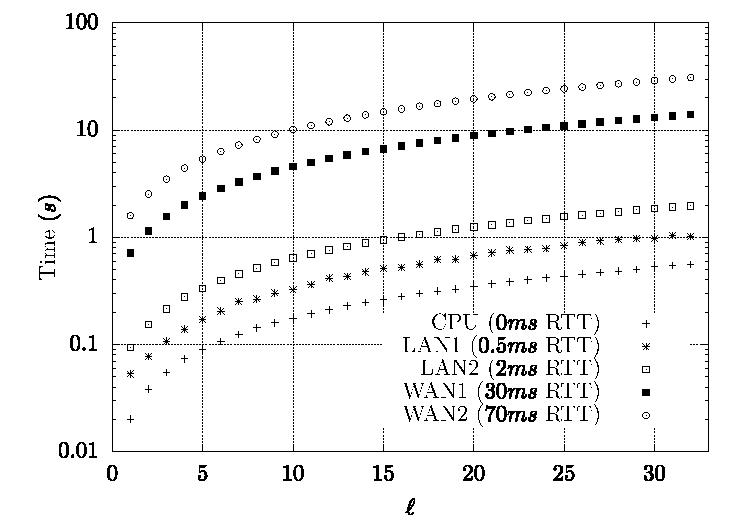
\includegraphics[width=\columnwidth]{plot.pdf}
  %\vspace*{-5mm}
  \caption{\label{figure}Total runtime of Construction~\ref{const:ioprf}}
\end{figure}
  \begin{table}[bb]\sisetup{detect-weight,mode=text}\small
    \centering\caption{\label{tab:imp}Cost breakdown}
    \sisetup{detect-weight,mode=text}
  \begin{tabular}{|c|cc|S[table-format=2.1]S[table-format=3.1]|cc|}
  \hline\multirow{2}{*}{$\ell$}& \multicolumn{2}{c|}{CPU (ms)}&\multicolumn{2}{c|}{Communication (kB)}&\multicolumn{2}{c|}{Total runtime (ms)}
  \\& Sender& Receiver & \multicolumn{1}{c}{Sender} & \multicolumn{1}{c|}{Receiver}& LAN1& WAN1
  \\\hline 5&44&41&11.7&26.1&171&2425
  \\10&88&81&23.2&51.4&325&4571
  \\15&126&123&34.6&76.6&512&6707
  \\20&174&162&46.1&101.9&679&8873
  \\25&218&202&57.5&127.1&836&10987
  \\30&267&248&69.0&152.4&968&13128
  \\\hline
\end{tabular}
\end{table}

To show practicality of Construction~\ref{const:ioprf} including its
ZK proofs, we have implemented and benchmarked its performance in
several realistic network settings. We stress that our implementation
is a full implementation of Construction~\ref{const:ioprf}, with all
Zero-Knowledge Proofs of Knowledge of Appendix~\ref{sec:sec-analysis},
i.e., including witness extractability and security against fully
malicious verifiers. Sender and receiver instances communicate via
standard TCP sockets.

Our implementation is done in $C$ and uses OpenSSL for elliptic curve
operations on NIST curve {\texttt{secp224r1}}. The source code is
available for download~\cite{srcode}.  We benchmark our implementation
on a 4.1~GHz Core i5-10600k.  As network latency is typically the
bottleneck in multi-round secure two-party computation protocols, we
benchmark Construction~\ref{const:ioprf} in different settings with
different network latencies.  To precisely control network latency
between sender and receiver instances, we use Linux' standard
{\texttt{tc-netem}} tool. Figure~\ref{figure} shows benchmark results
averaged over 50 executions, and Table~\ref{tab:imp} presents the cost
breakdown.

We measure total run time for values of $\ell$ ranging from $1$ to
$32$. Note that $\ell=32$ would support binary tree data structures
with $2^{32}$ different paths and $2^{33}-1$
(8.6~billion) nodes. We vary latency assuming LAN scenarios
with standard Gigabit Ethernet (0.5~ms RTT) or WiFi (2~ms RTT) and WAN
scenarios for intra-continental communication (30~ms RTT) and
inter-continental communication (70~ms RTT)~\cite{verizon}. We also
show an evaluation with 0~ms RTT, however even this number is still
dominated by the TCP communication overhead.  We found that the
computation alone in our protocol, including all EC computation and
ZKPs, is approximately 3~ms per $\ioprf$ iteration.

Each iOPRF evaluation for a tree data structure with $2^{20}$ nodes
needs about 170~ms of CPU time per party with our (unoptimized)
implementation.  As soon as we introduce higher latency, CPU time
contributes little to total runtime, and communication latency
becomes the main performance obstacle. For example, in the WAN1
scenario with intra-continental communication between sender and
receiver, total runtime is about 9~s of which less than $4\%$ is spent
with computation, and the remainder is consumed by network
latency.

We conclude from Figure~\ref{figure} that even for large values of
$\ell$ and for high latency network connections,
Construction~\ref{const:ioprf} has only a few seconds of runtime which
is practical for many scenarios.

In Appendix~\ref{sec:perf-related}, we discuss why alternative
approaches to realize the $\ioprf$ functionality perform worse than Construction~\ref{const:ioprf}.

\section{Applications}
\subsection{RFID}
We support a total of $N$ tags in the system. Each tag uniquely
corresponds to a leaf of a height $\ell$ (binary) key tree. To
identify a tag, a reader (a simple device which can query the tag and
has Internet connectivity) can talk to a database which knows all keys
of the key tree.

The reader wants to know whether a tag is valid by interacting first
with the tag and then with the database. To protect tag privacy,
internal details of a supply/distribution chain etc, the database
should not learn which tag the reader is querying for. An adversary
observing tag-reader interaction or being able to query tags
themselves should not be able to identify or trace/follow tags or
even fabricate new tags, too.


The database knows a secret key $K$ and populates a binary key tree
$T$ as follows. First, nodes in this key tree are indexed by bit
strings following the intuitive notation that the left child (``0'')
of some node indexed by bit string $\gamma_1\ldots\gamma_i$ is index by
$\gamma_1\ldots\gamma_i0$, and the right child (``1'') is indexed by
$\gamma_1\ldots\gamma_i1$. By convention, the root is indexed by
empty bit string $\epsilon$.

Root node $\epsilon$ stores random key
$K_{\epsilon}\getr\{0,1\}^\lambda$.  The left child of the root stores
key $K_0=\ioprf_K(0)$, and the right child stores key
$K_1=\ioprf_K(1)$. For a node $\gamma_1\ldots\gamma_i$,
the left child stores key
$K_{\gamma_1\ldots\gamma_i0}=\ioprf_K(\gamma_1\ldots\gamma_i0)$, and its
right child stores key
$K_{\gamma_1\ldots\gamma_i1}=\ioprf_K(\gamma_1\ldots\gamma_i1)$.

During authentication of tag $x$, the database will run
$\ioprf_K(\cdot)$ as the sender, and the reader will be the receiver
with input bit strings $x=x_1\ldots{}x_\ell$.

Here are protocol details.
\begin{itemize}
  
\item During initialization of a new tag $x$, the database stores a
  sequence of $\ell+1$ keys $K$ on the tag: one for each node on the
  path from the root of the database's tree $T$ to leaf
  $x=x_1\ldots{}x_\ell$. The tag also stores its own ID, i.e., $x$.

\item Each tag now identifies itself to a reader using a variation of
  the Molnar (\fixme{Difference: we send the next bit by appending
    it}) protocol:

  \begin{itemize}
  \item Tag $x$ chooses a random $r$ and sends $r$ together with a
    hash of $r$ and each of their $\ell+1$ keys and the next bit,
    respectively:
    $\trace=(r,T_0=H(r,
    K_\myroot,x_1),\ldots,T_\ell=H(r,K_{x_1\ldots{}x_{\ell-1}},x_{\ell}),H(r,K_{x_1\ldots{}x_\ell}))$.

\item The reader uses our $\ioprf$ to identify the tag as follows (I am now sticking to our running example of $x=1011$):

 \begin{itemize}

 \item The database beings by sending $K_\epsilon$ to the reader.
   
  \item The reader checks whether either $H(r,K_\epsilon,0)$ or $H(r,K_\epsilon,1)$  matches
    $T_0$.

  \item If yes, the reader would continue and query either the left or
    right child of the root with the $\ioprf$, compute keys, check
    which matches etc.
\end{itemize}
  \end{itemize}
\end{itemize}

As you can see, the security we are aiming for asks only for a
(delegatable) OPRF. Our $\ioprf$ supports delegation, but can do more. We
could also ask as an additional security requirement that the reader
should only learn ``one path'', i.e., one tag per interaction with the
database. 


\ignore{\newpage
section{This is the old protocol:}

Here are protocol details.
\begin{itemize}

\item During initialization of a new tag $x$, the database stores a
  sequence of $\ell$ keys $K$ on the tag, one for each node on the path from
  the root of the database's tree to leaf $x$. We keep the intuitive $0$
  and $1$ notation also for keys $K$, so for example tag $x = 1011$ stores
  keys $K_1$, $K_{10}$, $K_{101}$, $K_{1011}$, a total of $\ell=4$ keys.

\item The database computes each key as follows:  
\begin{itemize}
\item for a key corresponding to node $i$, it computes $\seed =
  \ioprf_K(\mathsf{PARENT}(i))$. For example, for $K_{1011}$, it would
  compute $\seed = \ioprf_K(101)$.

\item the database then computes
  $K_{\mathsf{leftChild}}||K_{\mathsf{rightChild}} = \prg(\seed)$. In
  our example, it would compute $K_{1010}||K_{1011} = \prg(\seed)$.

\item the database stores one of the two keys on the tag, the one corresponding to the node. So, $K_{1011}$ in our case.
\end{itemize}

\item Each tag can now identify itself to a reader using the Molnar protocol:

  \begin{itemize}
\item The tag chooses a random $r$ and sends $r$ together with a hash (or a PRF) of $r$ and each of their $\ell$ keys. So, it would send $r, H(r||K_1), H(r||K_{10}), H(r||K_{101}), H(r||K_{1011})$ to the reader.

\item The reader uses our $\ioprf$ to identify the tag as follows (I am now sticking to our running example of $x=1011$):
  \begin{itemize}
    
\item The reader would query the database for $\seed =
  \ioprf_K(\myroot)$, for some special input symbol $\myroot$.

\item The reader would derive $K_0$ and $K_1$ and would then check which of them matches the tag's first hash evaluation. 

\item If yes, the reader would continue and query either the left or right child of the root with the $\ioprf$, compute keys, check which hash matches etc.
\end{itemize}
  \end{itemize}
\end{itemize}

As you can see, the security we are aiming for asks only for a
delegatable OPRF. Our $\ioprf$ supports delegation, but can do more. We
could also ask as an additional security requirement that the reader
should only learn ``one path'', i.e., one tag per interaction with the
database. This is not 100\% true, because we currently also leak the
sibling of each ``key node'' in the above protocol. I don't think this
is a major problem though.
}%ignore

\subsubsection{Security Analysis}
{\bf Ideal Functionality $\myF$:}
We describe a reactive ideal functionality $\myF$.  The database sends
their input, keys $K_\myroot,K_0,K_1,\ldots,K_{1\ldots{}1}$, all $N$
keys of the key tree, to $\myF$, and the reader sends empty bit string
$\epsilon$. In return, $\myF$ sends $K_\myroot$ to the reader, and
nothing to the database.  The internal state $s$ of $\myF$ is
initialized to the empty bit string $\epsilon$.

Then, the RFID reader and $\myF$ additionally interact in a total of
$\ell$ rounds. In round $i$, let the internal state be bit string
$s=\beta_1\ldots{}\beta_{i-1}$. The reader sends bit $\beta_i$, and
$\myF$ responds with $K_{\beta_1\ldots\beta_{i}}$ and updates its
state to $s=\beta_1\ldots\beta_{i}$.


\paragraph{Proof}
\fixme{This seems trivial.}

\begin{proof}[Proof Draft]
  %For the proof, we assume that the RFID reader knows
  %$\trace=(r,H(r,
  %K_\myroot,x_1),\ldots,H(r,K_{x_1\ldots{}x_{\ell-1}},x_{\ell}),H(r,K_{x_1\ldots{}x_\ell}))$
  %from a valid tag $x$.

Public information: the total number $N$ of tags in the system (leaves
in tree $T$, $\lambda$ security parameter.

  \begin{enumerate}

  \item Simulator $\myS$ begins by preparing an initially empty
    key-value table $\mathsf{RO}$ to implement a standard random
    oracle functionality $H(\cdot)$. During simulation, whenever any
    party calls $H(k)$ for some input $k$, this functionality will
    check whether pair $(k,v)$ is already in table $\mathsf{RO}$ and
    responds with $v$ in that case. Otherwise, $H$ generates a random
    string $v$ of length $\lambda$, sends $v$ back to the caller, and
    places $(k,v)$ in $\mathsf{RO}$.

  \item Also, $\myS$ generates a random key
    $\kappa=((a_1,b_1),\ldots,(a_\ell,b_\ell))$ for $\ioprf$ and generates
    a common reference string including parameters which will allow
    $\myF$ to extract commitments from $\A$ (\fixme{be more formal,
    do some kind of GEN algorithm for iOPRF}).

  \item $\myS$ sends $\epsilon$ to $\myF$ and receives $K_\epsilon$
    which it forwards to $\A$.
    
  \item $\myS$ and $\A$ run $\proto$ with $\myS$ as the sender and
    $\A$ as the receiver.

    Recall that protocol $\proto$ runs iteratively with two messages
    exchanged between sender and receiver during each
    iteration. Consequently, $\A$ can adaptively choose their input
    bit $x_i$ for the $i^\text{th}$ iteration. The input of $\myS$ to
    $\proto$ is key $\kappa$.

    During the $i^\text{th}$ iteration\fixme{add check all ZK proofs
      etc}:
    \begin{enumerate}
    \item After receiving the first message in $\proto$, $\myS$
      extracts $\A$'s input $x_i$ from the Elgamal commitment,
      forwards it to $\myF$, and receives back $K_{x_1\ldots{}x_i}$.

    \item $\myS$ adds key-value pair
      $(( \prod_{j=1}^{i}
      a_j^{x_j}b_j^{1-x_j})\cdot{}G,K_{x_1\ldots{}x_i})$ to table
      $\mathsf{RO}$.
   
    \end{enumerate}
\end{enumerate}
\end{proof}



\section{Related Work}


\ignore{
\newpage

\section{Old}
\paragraph{Preliminaries} There are two parties $P_1$ and $P_2$ with
input sets $S_1=\{e_{1,1},\ldots,e_{1,n}\}$ and
$S_2=\{e_{2,1},\ldots,e_{2,n}\}$ of elements
$e_{i,j}\in\{0,1\}^\ell$. Both parties have agreed on an Elgamal key
pair $(pk,sk)$ where $sk$ is shared between the two of them.

For security parameter $\lambda$, there exists an oblivious
pseudo-random function
$\oprf:\{0,1\}^\lambda\times\{0,1\}^\ell\rightarrow{}\{0,1\}^\ell$.
In our context, $\oprf$ will be evaluated with $P_1$ being the sender
and $P_2$ being the receiver.

\paragraph{Protocol Overview}
\begin{enumerate}[label={\bf Step {\arabic*}:},leftmargin=*]
\item Party $P_1$ prepares a binary prefix tree of its input set as follows.

  First, $P_1$ generates a random key $k\getr\{0,1\}^\lambda$ for $\oprf$.

  For each $e_{1,i}\in{}S_1$, $P_1$ computes $V_i=\oprf_k(e_{1,i})$
  and builds a prefix tree $T$ with the $V_i$ as keys. Observe that
  each node $N_i$ in $T$ contains tuple
  $(\mathsf{prefix}_i,\mathsf{L}_i,\mathsf{R}_i)$, where
  $\mathsf{prefix}_i$ is node $N_i$'s bit string prefix, and
  $\mathsf{L}_i$ and $\mathsf{R}_i$ are pointers to the $N_i$'s left
  and right children and can therefore be $\bot$.

  $P_1$ stores $T$ in an array $A$, so pointers $\mathsf{L}_i$ and
  $\mathsf{R}_i$ are indices of $A$'s elements. Let the number
  of nodes in $T$ and therewith the number of elements in $A$ be
  $n'$.

  \fixme{Why would $P_1$ have to shuffle $T$?}
  
  Finally, $P_1$ Elgamal encrypts each element $N_i$ of array $A$ to
  $c_i=(\enc_{pk}(\mathsf{prefix}_i),\enc_{pk}(\mathsf{L}_i),\enc_{pk}(\mathsf{R}_i))$
  and sends the $c_i$ to $P_2$.

\item $P_2$ re-encrypts array $A$, i.e., all $c_i$ to $c'_i$, chooses
  a random permutation $\pi:\{1,\ldots,n\}\rightarrow\{1,\ldots,n\}$
  and randomly shuffles the $c'_i$ with $\pi$. Party $P_2$ sends
  resulting array $A'$, the sequence of $c'_{\pi(i)}$, back to $P_1$.

\item For each $e_{2,i}\in{}S_2$, $P_1$ and $P_2$ jointly evaluate
  $\oprf$ such that $P_2$ learns $v'_i=\oprf_k(e_{2,i})$, and $P_1$
  learns nothing.

\item Let $v'_i=b_{i,1}\ldots{}b_{i,\ell}$ be the bit representation
  of $v'_i$. Party $P_2$ fetches data from $P_1$ as follows.

  Party $P_2$ asks $P_1$ to partially decrypt element $\pi(0)$, the
  root, from $A'$. Upon receipt, $P_2$ finalizes decryption of
  $\pi(0)$ to $(\mathsf{prefix},\mathsf{L},\mathsf{R})$.

  They then use bit $b_{i,1}$ to either set
  ${\mathsf{next}}=\mathsf{L}$ or ${\mathsf{next}}=\mathsf{R}$, fetch
  the partial decryption of $\pi({\mathsf{next}})$ from $A'$ and so on.

  Note that $P_2$ never fetches the same element from $A'$ twice. 
  
\end{enumerate}

\fixme{Optimization: do not send back the shuffled array...}

\section{Related Work}
\begin{itemize}
\item Katzenbeisser: \url{https://dl.acm.org/doi/pdf/10.1145/1315245.1315309}:
  privacy-preserving evaluation of a FSM, semi-honest, number of
  states (and therewith this scheme's communication complexity) of the
  FSM is exponential in the edit distance:
  \url{https://store.fmi.uni-sofia.bg/fmi/logic/theses/mitankin-en.pdf}
\item Kerschbaum: \url{http://citeseerx.ist.psu.edu/viewdoc/download?doi=10.1.1.584.3879&rep=rep1&type=pdf}, semi-honest, $\ell^2$ per item
\end{itemize}
}%ignore



\section{Difference to structured encryption}
\begin{itemize}
\item Different adversary model
\item Matrix queries and labeled data queries, neighbor queries and adjacency queries on graphs, are trivial.
\item Token length?!
\item the original PRF is mentioned by Naor and Reingold (Section 6.3), but details on how to use OT is mentioned by \url{https://www.iacr.org/archive/tcc2005/3378_304/3378_304.pdf}.  
\end{itemize}



\ignore{
* Note that our iOPRF can be evaluated ``interactively'',  i.e., the receiver runs OTs adaptively

Motivation:

* One could just replace the PRF in structured encryption (Figure 2 /
Section 5) with an OPRF, but this is not sufficient: the adversary
could ``flip-flop'' inside the graph, but we want that they can only
follow paths.


Apps:
* Graphs: https://robobees.seas.harvard.edu/files/privacytools/files/grecs.pdf
and https://par.nsf.gov/servlets/purl/10042572 and http://www.vldb.org/pvldb/vol11/p420-sahu.pdf

* Similar as with structured encryption (web graphs, graphs, matrices)

* What about running SQL queries https://eprint.iacr.org/2016/453.pdf

* We also allow for ``controlled disclosure'', e.g., the server
reveals one internal node, the root of some subtree, and the client
can then go on and make queries on that subtree. 

https://www.cis.upenn.edu/~mkearns/papers/nwlocal.pdf
Jump and crawl algorithms for analyzing social networks

* Microsoft Azure Marketplace: allow a cloud application to analyze your data.
** Data provider does not want to reveal whole data set, but only ``subtree''
** Cloud Application does not want to leak details about their techniques 
*** Compromise between no security and fully-homomorphic encryption or MPC

* HITS and PageRank: algorithms to analyze properties of an intranet, local sub-tree of the intranet

}



\bibliographystyle{plainnat}
\bibliography{main}
\end{document}
